% vim:ts=4:sw=4
% Copyright (c) 2014 Casper Ti. Vector
% Public domain.

\chapter{毫秒脉冲星的多波段脉冲偏振轮廓图片}

\begin{figure*}
\begin{center}
\includegraphics[width=6 in]{0437.ps}
\caption{PSR J0437$-$4715的多波段偏振轮廓和相位分离研究.}
\label{0437}
\end{center}
\end{figure*}

\begin{figure*}
\begin{center}
\includegraphics[width=6 in]{0613.ps}
\caption{PSR J0613$-$0200的多波段偏振轮廓和相位分离研究.}
\label{0613}
\end{center}
\end{figure*}

\begin{figure*}
\begin{center}
\includegraphics[width=6 in]{0711.ps}
\caption{PSR J0711$-$6830的多波段偏振轮廓和相位分离研究.}
\label{0711}
\end{center}
\end{figure*}

\begin{figure*}
\begin{center}
\includegraphics[width=6 in]{1017.ps}
\caption{PSR J1017$-$7156的多波段偏振轮廓和相位分离研究.}
\label{1017}
\end{center}
\end{figure*}

\begin{figure*}
\begin{center}
\includegraphics[width=6 in]{1022.ps}
\caption{PSR J1022$+$1001的多波段偏振轮廓和相位分离研究.}
\label{1022}
\end{center}
\end{figure*}

\begin{figure*}
\begin{center}
\includegraphics[width=6 in]{1024.ps}
\caption{PSR J1024$-$0719的多波段偏振轮廓和相位分离研究.}
\label{1024}
\end{center}
\end{figure*}

\begin{figure*}
\begin{center}
\includegraphics[width=6 in]{1045.ps}
\caption{PSR J1045$-$4509的多波段偏振轮廓和相位分离研究.}
\label{1045}
\end{center}
\end{figure*}

\begin{figure*}
\begin{center}
\includegraphics[width=6 in]{1446.ps}
\caption{PSR J1446$-$4701的多波段偏振轮廓和相位分离研究.}
\label{1446}
\end{center}
\end{figure*}

\begin{figure*}
\begin{center}
\includegraphics[width=6 in]{1545.ps}
\caption{PSR J1545$-$4550的多波段偏振轮廓和相位分离研究.}
\label{1545}
\end{center}
\end{figure*}

\begin{figure*}
\begin{center}
\includegraphics[width=6 in]{1600.ps}
\caption{PSR J1600$-$3053的多波段偏振轮廓和相位分离研究.}
\label{1600}
\end{center}
\end{figure*}

\begin{figure*}
\begin{center}
\includegraphics[width=6 in]{1603.ps}
\caption{PSR J1603$-$7202的多波段偏振轮廓和相位分离研究.}
\label{1603}
\end{center}
\end{figure*}

\begin{figure*}
\begin{center}
\includegraphics[width=6 in]{1643.ps}
\caption{PSR J1643$-$1224的多波段偏振轮廓和相位分离研究.}
\label{1643}
\end{center}
\end{figure*}

\begin{figure*}
\begin{center}
\includegraphics[width=6 in]{1713.ps}
\caption{PSR J1713$+$0747的多波段偏振轮廓和相位分离研究.}
\label{1713}
\end{center}
\end{figure*}

\begin{figure*}
\begin{center}
\includegraphics[width=6 in]{1730.ps}
\caption{PSR J1730$-$2304的多波段偏振轮廓和相位分离研究.}
\label{1730}
\end{center}
\end{figure*}

\begin{figure*}
\begin{center}
\includegraphics[width=6 in]{1744.ps}
\caption{PSR J1744$-$1134的多波段偏振轮廓和相位分离研究.}
\label{1744}
\end{center}
\end{figure*}

\begin{figure*}
\begin{center}
\includegraphics[width=6 in]{1824.ps}
\caption{PSR J1824$-$2452的多波段偏振轮廓和相位分离研究.}
\label{1824}
\end{center}
\end{figure*}

\begin{figure*}
\begin{center}
\includegraphics[width=6 in]{1832.ps}
\caption{PSR J1832$-$0836的多波段偏振轮廓和相位分离研究.}
\label{1832}
\end{center}
\end{figure*}

\begin{figure*}
\begin{center}
\includegraphics[width=6 in]{1857.ps}
\caption{PSR J1857$+$0943的多波段偏振轮廓和相位分离研究.}
\label{1857}
\end{center}
\end{figure*}

%\clearpage

\begin{figure*}
\begin{center}
\includegraphics[width=6 in]{1909.ps}
\caption{PSR J1909$-$3744的多波段偏振轮廓和相位分离研究.}
\label{1909}
\end{center}
\end{figure*}

\begin{figure*}
\begin{center}
\includegraphics[width=6 in]{1939.ps}
\caption{PSR J1939$+$2134的多波段偏振轮廓和相位分离研究.}
\label{1939}
\end{center}
\end{figure*}

\begin{figure*}
\begin{center}
\includegraphics[width=6 in]{2124.ps}
\caption{PSR J2124$-$3358的多波段偏振轮廓和相位分离研究.}
\label{2124}
\end{center}
\end{figure*}

\begin{figure*}
\begin{center}
\includegraphics[width=6 in]{2129.ps}
\caption{PSR J2129$-$5721的多波段偏振轮廓和相位分离研究.}
\label{2129}
\end{center}
\end{figure*}

\begin{figure*}
\begin{center}
\includegraphics[width=6 in]{2145.ps}
\caption{PSR J2145$-$0750的多波段偏振轮廓和相位分离研究.}
\label{2145}
\end{center}
\end{figure*}

\begin{figure*}
\begin{center}
\includegraphics[width=6 in]{2241.ps}
\caption{PSR J2241$-$5236的多波段偏振轮廓和相位分离研究.}
\label{2241}
\end{center}
\end{figure*}

\pkuthssffaq

